\documentclass{beamer}
%
% Choose how your presentation looks.
%
% For more themes, color themes and font themes, see:
% http://deic.uab.es/~iblanes/beamer_gallery/index_by_theme.html
%
\mode<presentation>
{
  \usetheme{default}      % or try Darmstadt, Madrid, Warsaw, ...
  \usecolortheme{default} % or try albatross, beaver, crane, ...
  \usefonttheme{default}  % or try serif, structurebold, ...
  \setbeamertemplate{navigation symbols}{}
  \setbeamertemplate{caption}[numbered]
  \setbeamertemplate{footline}[frame number]
} 

\usepackage[english]{babel}
\usepackage[utf8x]{inputenc}
\usepackage{dirtree}
\usepackage{listings}
\usepackage{courier}
\usepackage{array}

\title[2016-04-04-offline-pr-overview]{Big Data techniques and \\ applying them to high energy physics}
\author{Jim Pivarski}
\institute{Princeton University -- DIANA}
\date{April 4, 2016}

\xdefinecolor{darkblue}{rgb}{0.1,0.1,0.7}
\definecolor{mygreen}{rgb}{0,0.6,0}
\definecolor{mygray}{rgb}{0.5,0.5,0.5}
\definecolor{mymauve}{rgb}{0.58,0,0.82}
\xdefinecolor{darkgrey}{rgb}{0.35,0.35,0.35}

\lstset{ %
  backgroundcolor=\color{white},   % choose the background color
  basicstyle=\ttfamily\scriptsize,        % size of fonts used for the code
  breaklines=true,                 % automatic line breaking only at whitespace
  captionpos=b,                    % sets the caption-position to bottom
  commentstyle=\color{mygreen},    % comment style
  escapeinside={\%*}{*)},          % if you want to add LaTeX within your code
  keywordstyle=\color{blue},       % keyword style
  stringstyle=\color{mymauve},     % string literal style
  showstringspaces=false,
  showlines=true
}

\lstdefinelanguage{scala}{
  morekeywords={abstract,case,catch,class,def,%
    do,else,extends,false,final,finally,%
    for,if,implicit,import,match,mixin,%
    new,null,object,override,package,%
    private,protected,requires,return,sealed,%
    super,this,throw,trait,true,try,%
    type,val,var,while,with,yield},
  otherkeywords={=>,<-,<\%,<:,>:,\#,@},
  sensitive=true,
  morecomment=[l]{//},
  morecomment=[n]{/*}{*/},
  morestring=[b]",
  morestring=[b]',
  morestring=[b]"""
}

\begin{document}

\begin{frame}
  \titlepage
\end{frame}

% Uncomment these lines for an automatically generated outline.
%\begin{frame}{Outline}
%  \tableofcontents
%\end{frame}

\begin{frame}{How did I end up giving this talk?}
\begin{itemize}
\item I'm a CMS physicist, contributed to muon alignment in Run-1 commissioning and early exotica searches.
\item Spent the next five years as a data science consultant:
\begin{itemize}
\item Helped commercial clients analyze data with Big Data technologies: Hadoop, Spark, NoSQL, etc.
\item Some statistics, but more software and data pipelines.
\end{itemize}
\end{itemize}

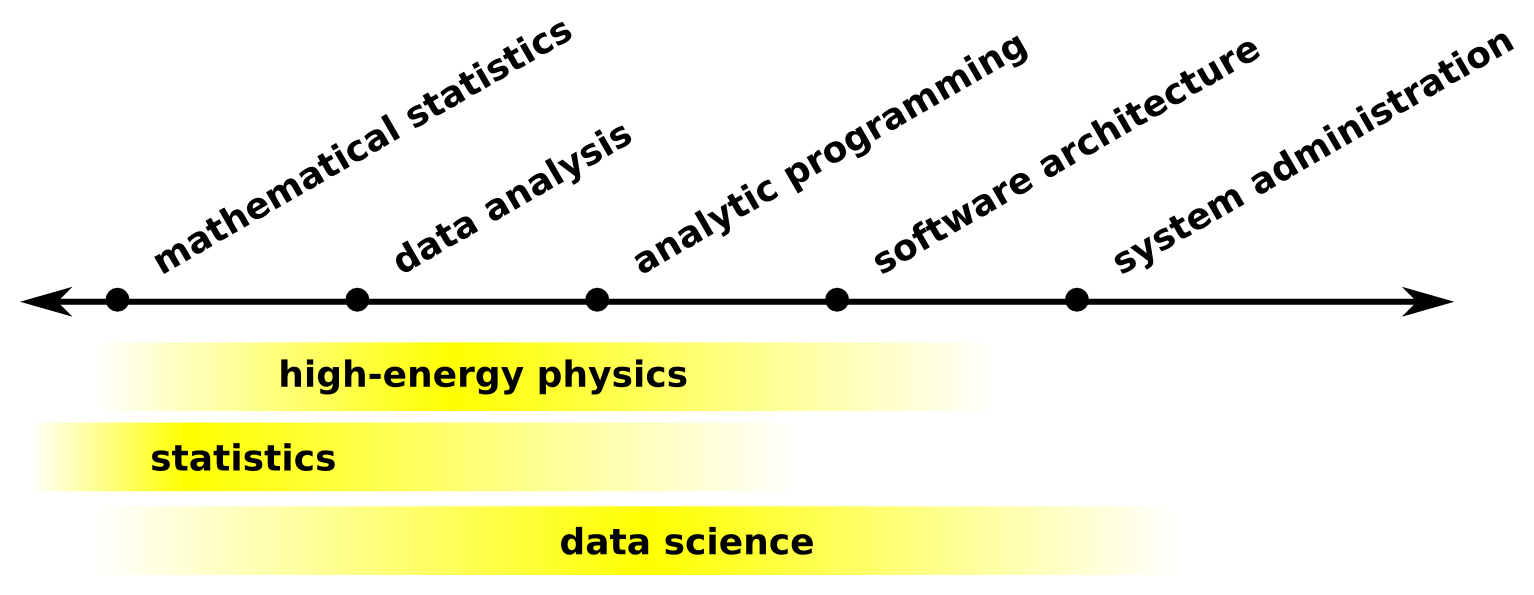
\includegraphics[width=\linewidth]{spectrum_of_data_science.png}

\uncover<2->{\fbox{\parbox{\linewidth}{Now I'm part of a project to introduce Big Data tools to HEP. \\ \centering \url{http://diana-hep.org}}}}
\end{frame}

\begin{frame}{Differences between HEP and the Big Data world}
\begin{columns}
\column{0.5\linewidth}
\centering \textcolor{darkblue}{HEP}

\column{0.5\linewidth}
\centering \textcolor{darkblue}{Big Data}
\end{columns}

\vfill
\begin{columns}
\column{0.5\linewidth}
One integrated toolkit: ROOT. Compared to a ``city with central services'' in the User's Guide.

\column{0.5\linewidth}
Many competing frameworks and data formats that nevertheless interoperate: ``city-states?''
\end{columns}

\vfill
\uncover<2->{\hrulefill}

\vfill
\begin{columns}<2->
\column{0.5\linewidth}
C++ for data plumbing and (increasingly) Python for end-user analysis.

\column{0.5\linewidth}
Java for data plumbing and (mostly) Python, R, and SQL for analysis.
\end{columns}

\vfill
\uncover<3->{\hrulefill}

\vfill
\begin{columns}<3->
\column{0.5\linewidth}
Extensive distributed filtering \\ and data transformations \\ (the ``map'' of map-reduce).

\column{0.5\linewidth}
Extensive distributed map {\it and} reduce: regrouping data from one lookup key to another.
\end{columns}

\vfill
\uncover<4->{\hrulefill}

\vfill
\begin{columns}<4->
\column{0.5\linewidth}
Data analysis mostly written imperatively: for loops, break/continue statements.

\column{0.5\linewidth}
Increasing use of functional primitives: map, filter, flatMap, reduce, aggregate.
\end{columns}
\end{frame}

\vfill
\begin{frame}{The ecosystem}
\vspace{-0.6 cm}
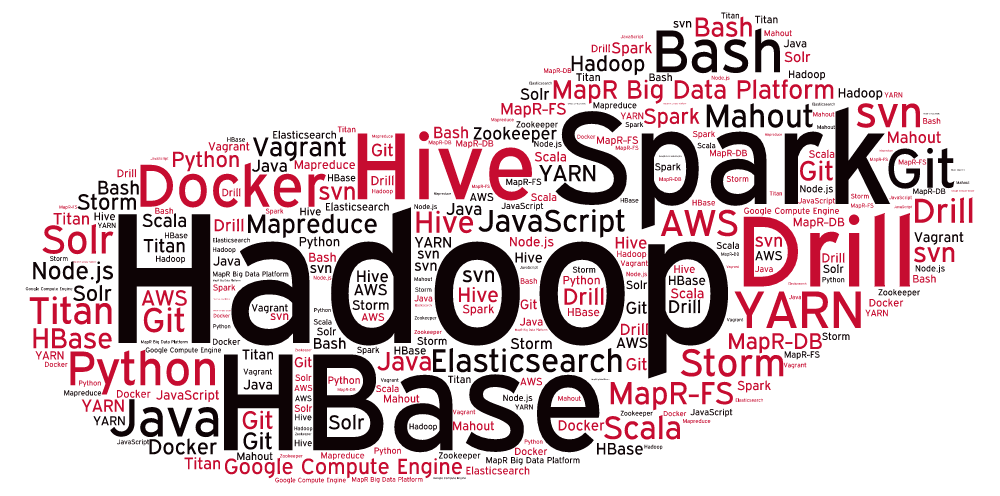
\includegraphics[width=\linewidth]{word-cloud-07-2014.png}

\begin{onlyenv}<2->
\vspace{0.5 cm}
\begin{columns}
\column{0.5\linewidth}
KDNuggets poll results:

\vspace{0.1 cm}
{\scriptsize
\begin{itemize}
\item Hadoop, 18.4\% share (507 votes)
\item Spark, 11.3\% (311)
\item Hive, 10.2\% (282)
\item SQL on Hadoop tools, 7.2\% (198)
\item Others, 21.4\% (592)
\end{itemize}}

\column{0.5\linewidth}
Google Trends search popularity:

\vspace{0.5 cm}
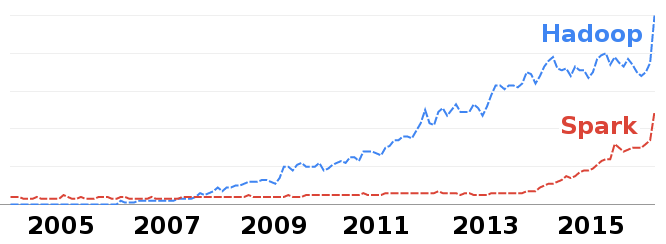
\includegraphics[width=\linewidth]{trends.png}
\end{columns}
\end{onlyenv}
\end{frame}

\begin{frame}{Diversity: just to make a point}

There are FIVE stream-processing systems maintained by Apache:

\begin{center}
\begin{minipage}{0.8\linewidth}
\begin{center}

\includegraphics[width=0.4\linewidth]{streaming-1.png} \hfill

\includegraphics[width=0.4\linewidth]{streaming-2.png}

\vspace{0.2 cm}

\includegraphics[width=0.5\linewidth]{streaming-3.png}

\vspace{0.2 cm}

\includegraphics[width=0.4\linewidth]{streaming-4.png} \hfill

\includegraphics[width=0.4\linewidth]{streaming-5.jpg}
\end{center}
\end{minipage}
\end{center}

\vfill
They all do the same thing as far as I can tell. One will emerge as the most popular and get the most contributions (either Storm or Spark-Streaming).
\end{frame}

\begin{frame}{File formats: more ways of doing the same thing}

\vfill
\hspace{-0.4 cm}\begin{minipage}{\linewidth}
\renewcommand{\arraystretch}{1.5}
\begin{tabular}{p{0.4\linewidth} p{0.6\linewidth}}
\textcolor{darkblue}{JSON, XML, CSV\ldots} & Text-based for human readability; more common than you'd think. \\
\raggedright \textcolor{darkblue}{Avro, Thrift, Protocol buffers\ldots} & Generic, row-based binary data, like JSON with a schema. \\
\textcolor{darkblue}{Parquet, ORC, RCFile\ldots} & Generic, columnar binary data, used for SQL-style analyses. \\
\raggedright \textcolor{darkblue}{Java serialization, Kryo, Hadoop Writables\ldots} & Intermediate serialization for data in a distributed stream. \\
\textcolor{darkblue}{Python pickle files} & Persist Python objects between sessions. \\
\textcolor{darkblue}{RData, RDS} & Persist R objects between sessions. \\
\end{tabular}
\end{minipage}
\vfill

But there are plenty of adapters from one format to another.
\vfill
\end{frame}

\begin{frame}{}
\begin{center}
\begin{minipage}{0.8\linewidth}
It's obvious why HEP hasn't chosen this model: who could maintain so many alternatives?

\vspace{1.5 cm}
But perhaps we can use what's out there and let the Big Data community maintain it.

\vspace{1.5 cm}
Almost everything is available through the standard package managers (Maven Central, PyPI, CRAN, \ldots).
\end{minipage}
\end{center}
\end{frame}

\begin{frame}{The C++/Java barrier}

\vspace{0.2 cm}
One thing most of these toolkits have in common is that they are written for the Java Virtual Machine (JVM). This is hard to bridge.

\begin{center}
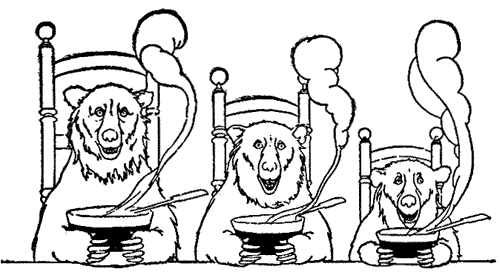
\includegraphics[width=0.5\linewidth]{three_bears.png}
\end{center}

\renewcommand{\arraystretch}{1.2} \begin{tabular}{>{\raggedright}p{0.23\linewidth} >{\raggedright}p{0.35\linewidth} >{\raggedright\arraybackslash}p{0.33\linewidth}}
\textcolor{darkblue}{C/C++} & \textcolor{darkblue}{JVM (Java, Scala\ldots)} & \textcolor{darkblue}{Python and R} \\
\vspace{-0.4 cm} Fast, but hard to debug. & \vspace{-0.4 cm} Type-aware bytecode is moderately fast. & \vspace{-0.4 cm} Offload heavy work to precompiled packages. \\
Mixes analysis with hardware concerns. & High-level abstractions for data analysis, but better geared toward batch processes. & Highly interactive; ideal the compute- plot-think cycle.
\end{tabular}
\end{frame}

\begin{frame}{}
\vfill
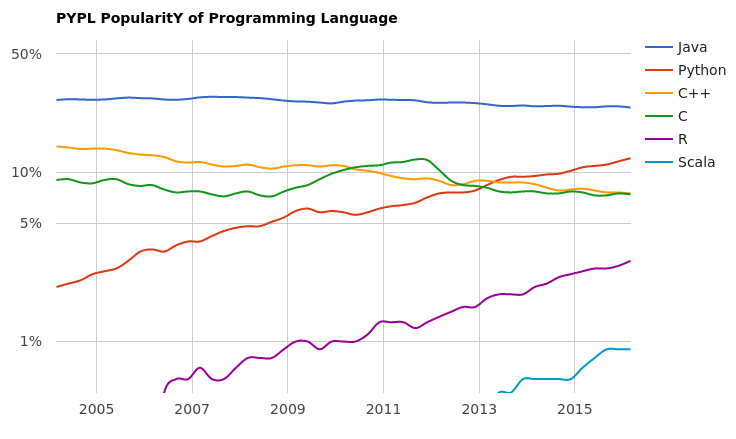
\includegraphics[width=\linewidth]{language_trends.png}

\vfill
Warning: different trend analyses vary by $\sim$15\%.
\end{frame}

\begin{frame}{}
\vfill
More specifically: what languages are used for data analytics?

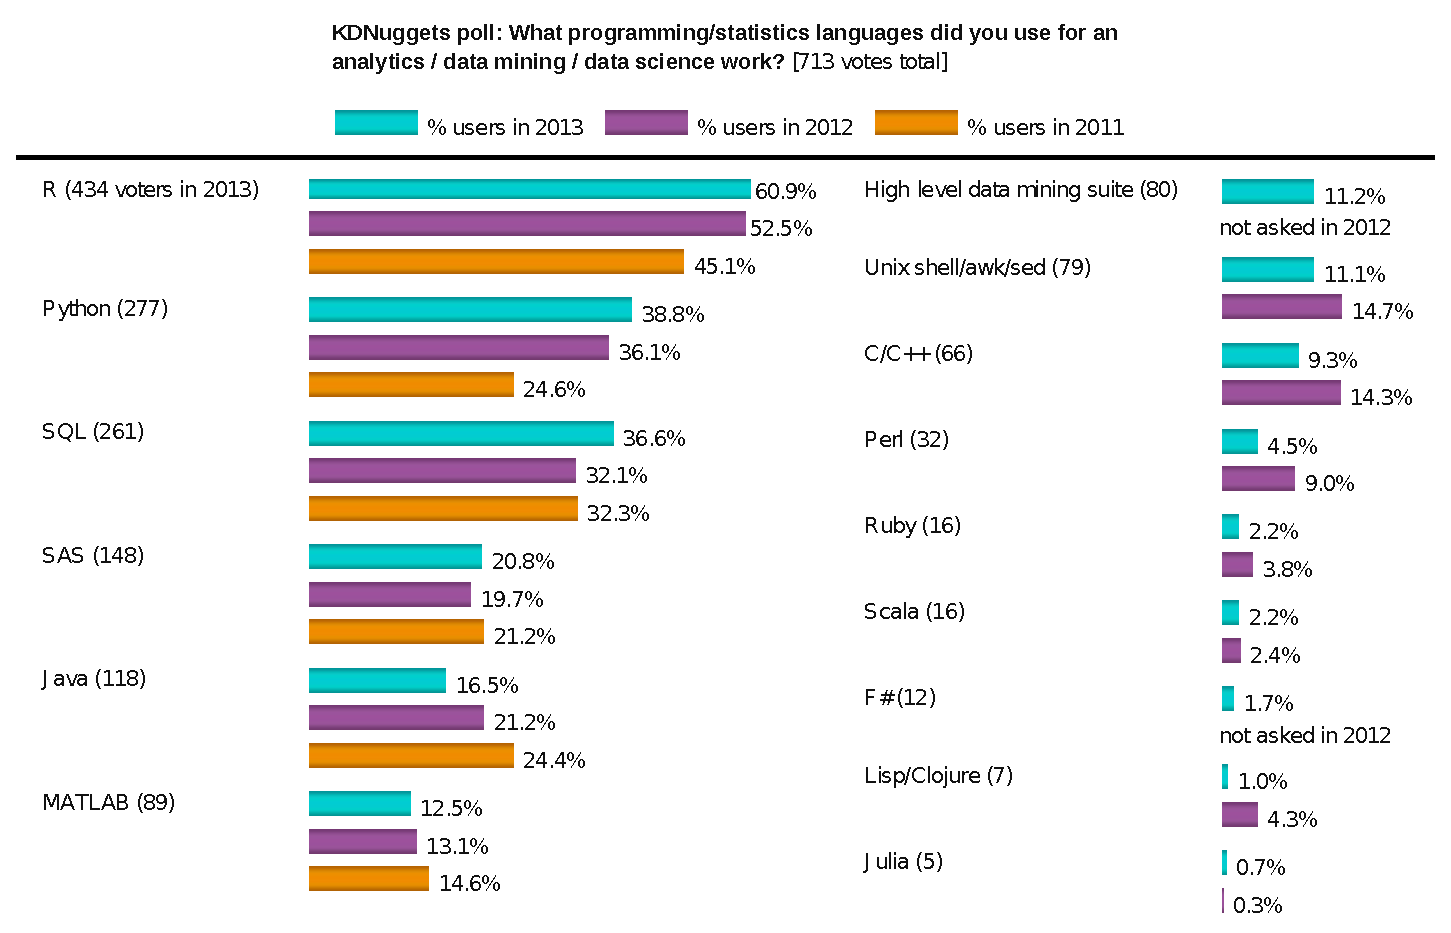
\includegraphics[width=\linewidth]{KDNuggetsPoll.pdf}

\vfill
\scriptsize (2013 KDNuggets poll)
\end{frame}

\begin{frame}{Overcoming the C++/Java barrier}

\begin{itemize}
\item Python and R have extension modules to call compiled code.
\item Java has its JNI (Java Native Interface), but it is {\it much less} used. (Except among high-frequency traders.)
\end{itemize}

\begin{uncoverenv}<2->
\begin{block}{}
\vspace{-\baselineskip}
I have been developing adapters to connect ROOT with the JVM so that we can use Big Data tools in our physics analyses.

\begin{itemize}
\item \textcolor{darkgrey}{Using JNI so that C++ code and Java run in the same process (no interprocess communication).}
\item \textcolor{darkgrey}{Arbitrarily complex ROOT TTrees to include CMSSW objects.}
\item \textcolor{darkgrey}{ROOT does file I/O to inherit XRootD abilities.}
\item \textcolor{darkgrey}{Scala interface, rather than pure Java, to target Spark.}
\item \textcolor{darkgrey}{Scala macros ``compile in'' data type information for speed.}
\item \only<2>{\textcolor{darkgrey}{Combining Scala macros with ROOT's Cling interface to create Java interfaces with C++ implementations.}}\only<3>{Combining Scala macros with ROOT's Cling interface to create Java interfaces with C++ implementations.}
\end{itemize}
\end{block}
\end{uncoverenv}
\end{frame}

\begin{frame}{ScaROOT: Java interfaces with C++ implementations}

\vfill
\fbox{\url{http://github.com/diana-hep/scaroot}}

\vfill
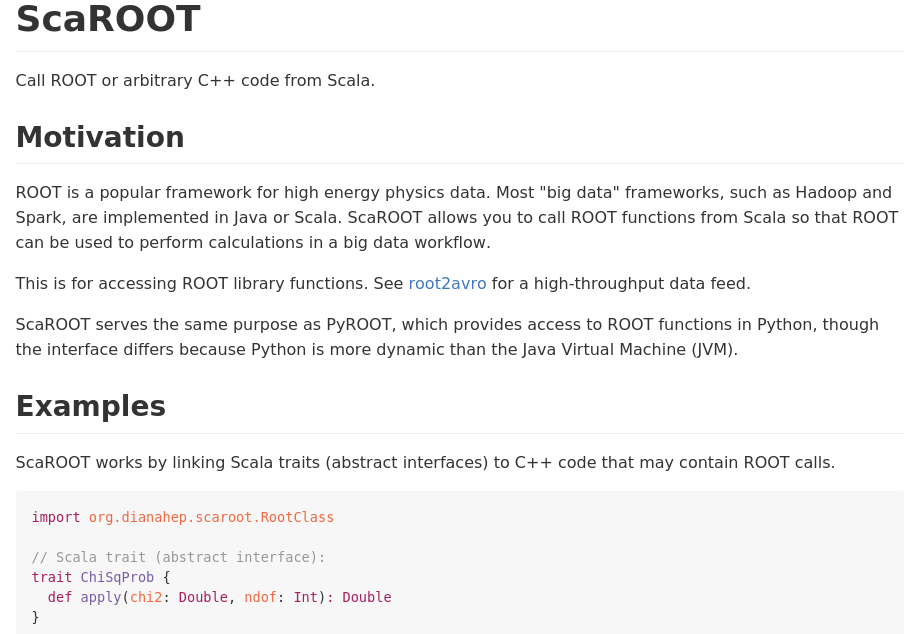
\includegraphics[width=\linewidth]{wiki.png}
\end{frame}

\begin{frame}[fragile]{ScaROOT: Java interfaces with C++ implementations}
\begin{lstlisting}[language=scala]
import org.dianahep.scaroot.RootClass

// Java interface (called a "trait" in Scala):
trait ChiSqProb {
  def apply(chi2: Double, ndof: Int): Double
}

// C++ class definition that satisfies this interface:
val chiSqProbClass = RootClass[ChiSqProb]("""
class ChiSqProb {
public:
  double apply(double chi2, int ndof) {
    return ROOT::Math::chisquared_cdf(chi2, ndof);
  }
};
""")

// Create an instance:
val chiSqProb = chiSqProbClass.newInstance

// And use it:
chiSqProb.apply(53.8, 50)   // or just chiSqProb(53.8, 50)
                            // because 'apply' is 'operator()'
0.6689797343068249
\end{lstlisting}
\end{frame}

\begin{frame}[fragile]{ScaROOT-Reader: accessing ROOT TTrees}
\vfill
\fbox{\url{http://github.com/diana-hep/rootconverter}}

\vfill
\begin{minipage}{1.05\linewidth}
\begin{lstlisting}[language=scala]
// Define a concrete class for data to go into:
case class TwoMuon(mass: Float, px: Float, py: Float, pz: Float) {
  def pt = Math.sqrt(px*px + py*py)
}

// The brackets (equivalent of C++ template) generates custom
// data-filling code with a compile-time macro.
val iterator = RootTreeIterator[TwoMuon](
  List("root://cmseos.fnal.gov/TwoMuonNtuple.root"), "twoMuon")

// Do anything with this data stream in the JVM.
while (iterator.hasNext) {
  val datum = iterator.next()
  println(s"mass: ${datum.mass} pt: ${datum.pt}")
}
\end{lstlisting}
\end{minipage}

Also includes a pure-C++ {\tt root2avro} for streaming or bulk file conversion without involving the JVM.
\end{frame}

\begin{frame}[fragile]{Complex example: Bacon-tuple as an Avro schema}
\tiny
\begin{verbatim}
{"type": "record",
 "name": "Events",
 "fields": [
   {"name": "GenParticle", "type": {"type": "array", "items": {"type": "record",
    "name": "TGenParticle",
    "namespace": "baconhep",
    "fields": [
      {"name": "parent", "type": "int"},
      {"name": "pdgId", "type": "int"},
      {"name": "status", "type": "int"},
      {"name": "pt", "type": "float"},
      {"name": "eta", "type": "float"},
      {"name": "phi", "type": "float"},
      {"name": "mass", "type": "float"},
      {"name": "y", "type": "float"}
    ]
   }}},
   {"name": "LHEWeight", "type": {"type": "array", "items": {"type": "record",
    "name": "TLHEWeight",
    "namespace": "baconhep",
    "fields": [
      {"name": "id", "type": "int", "doc": "parton flavor PDG ID"},
      {"name": "weight", "type": "float", "doc": "generator-level event weight"}
    ]
   }}},
   {"name": "Electron", "type": {"type": "array", "items": {"type": "record",
    "name": "TElectron",
    "namespace": "baconhep",
    "fields": [
      {"name": "pt", "type": "float", "doc": "kinematics"},
      {"name": "eta", "type": "float", "doc": "kinematics"},
      {"name": "phi", "type": "float", "doc": "kinematics"},
      ...
\end{verbatim}
\end{frame}

\begin{frame}[fragile]{}
\hspace{-0.6 cm}ScaROOT-Reader is being used in a CMS monojet analysis:
\begin{columns}
\column{0.6\linewidth}
\begin{itemize}
\item Oliver Gutsche
\item Matteo Cremonesi
\item Cristina Su\'arez (made plot at right from a Bacon-tuple in Spark)
\end{itemize}

\vspace{0.5 cm}
Part of a wider Big Data-in-HEP effort:
\begin{itemize}
\item Alexey Svyatkovskiy (Princeton)
\item Saba Sehrish and Jim Kowalkowski (FNAL Scientific Computing)
\end{itemize}
\column{0.5\linewidth}
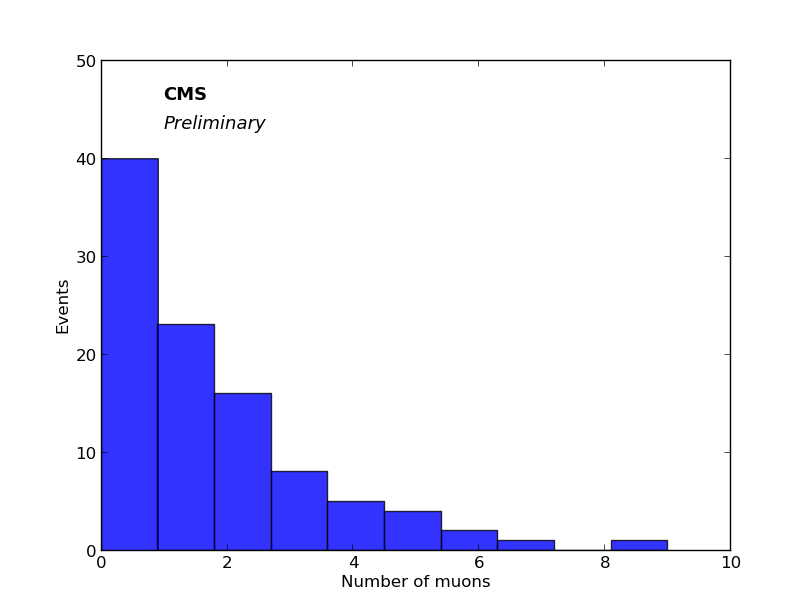
\includegraphics[width=\linewidth]{THE_PLOT.png}
\end{columns}

\vspace{0.5 cm}
\begin{uncoverenv}<2->
\hspace{-0.6 cm}Producing a distributed TTree iterator in Spark:

\begin{lstlisting}[language=scala]
val rdd = file_list.flatMap(files => RootTreeIterator[Tree](
  files.map(_.xrootd_url), tree_location, libs, class_links))

rdd.map(...).filter(...).reduce(...)
\end{lstlisting}
\end{uncoverenv}
\end{frame}

\begin{frame}{}
\vfill
\textcolor{darkblue}{\Large So we can run physics events through Big Data \mbox{tools.\hspace{-1 cm}}}

\vspace{0.3 cm}
\textcolor{darkblue}{\Large What does that buy us?}

\begin{uncoverenv}<2->
\begin{itemize}\setlength{\itemsep}{0.2 cm}
\item Code maintained by large open-source organizations like Apache.
\item More complex forms of distributed data processing, such as the ``reduce'' step in map-reduce.
\item Resilient stream processing for data quality monitoring.
\item Higher data-handling abstractions, which analysts in other fields are already benefiting from.
\end{itemize}
\end{uncoverenv}
\end{frame}

\begin{frame}{Workflow coupling}

\begin{block}{Most physics analyses}
Uncoupled: to process one event, you don't need to know anything about any other events.
\end{block}

\begin{block}{Most industrial problems}
Require large datasets to be transposed, regrouping distributed data from one lookup key to another. Tightly coupled.
\end{block}

\begin{uncoverenv}<2->
\begin{block}{Example}
\begin{itemize}
\item A customer buys diapers online; what other products should you recommend?
\item Analysis of diaper purchases across {\it all customers} reveals a correlation with milk, so recommend milk.
\end{itemize}
\end{block}
\end{uncoverenv}
\end{frame}

\begin{frame}{}
\begin{block}{Example}
\begin{itemize}
\item A customer buys diapers online; what other products should you recommend?
\item Analysis of diaper purchases across {\it all customers} reveals a correlation with milk, so recommend milk.
\end{itemize}
\end{block}

\vfill
\textcolor{darkblue}{Customer records need to be split and grouped by purchase items.}

\begin{center}
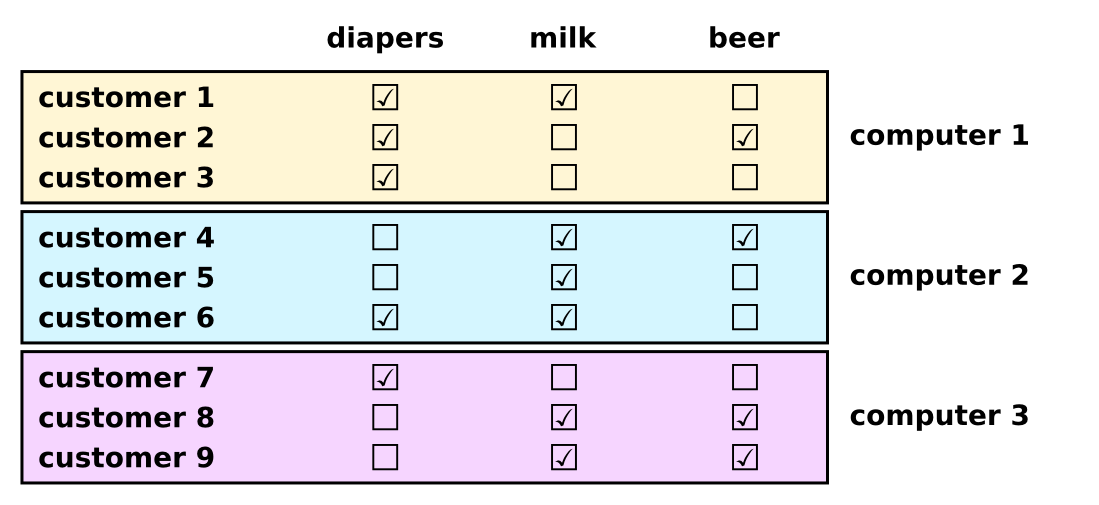
\includegraphics[width=0.9\linewidth]{distributed_data.png}
\end{center}
\end{frame}

\begin{frame}[fragile]{This was Google's problem: solved with map-reduce}

Must reindex data from words-in-webpages to \mbox{webpages-with-words.\hspace{-1 cm}}

\begin{columns}
\column{0.5\linewidth}
\begin{lstlisting}[language=python,frame=single]
def mapper(webpage):
    for word in webpage.split():
        yield (word, webpage)
    
\end{lstlisting}
\column{0.58\linewidth}
\begin{lstlisting}[language=python,frame=single]
def reducer(word, webpages):
   searchIndex[word] = set()
   for webpage in webpages:
       searchIndex[word].add(webpage)
\end{lstlisting}
\end{columns}

\begin{itemize}
\item Independent mappers transform input to $\langle$key, value$\rangle$ pair.
\item Each reducer is given {\it all} pairs with a unique key.
\item Map-reduce framework optimizes the sorting and merging required to collect unique keys.
\end{itemize}

\begin{center}
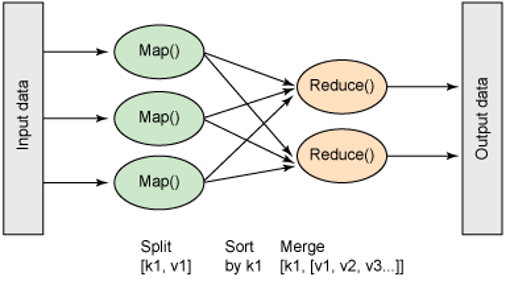
\includegraphics[width=0.65\linewidth]{mapreduce-diagram-by-ibm.png}
\end{center}
\end{frame}

\begin{frame}[fragile]{Physics application: track alignment iteration}

Must reindex data from residuals-on-tracks to \mbox{residuals-on-subdetectors.\hspace{-1 cm}}

\vfill
\begin{lstlisting}[language=python,frame=single]
def mapper(event):
    for track in event:
        for hit in track:
            key = hit.subdetector()
            residual = track.projection(hit) - hit.position()
            yield (key, residual)
\end{lstlisting}

\begin{lstlisting}[language=python,frame=single]
def reducer(subdetector, residuals):
    numer = 0
    denom = 0
    for residual in residuals:
        numer = numer + residual
        denom = denom + 1
    move(subdetector, numer/denom)  # shift by residual mean
\end{lstlisting}

\vfill
\begin{itemize}
\item Applies broadly to many alignment and calibration tasks (e.g. reindex from energy-in-$\pi^0$ to energy-in-crystal).
\item Currently, detector groups are reimplementing this in custom ways, using tools designed for uncoupled event processing.
\end{itemize}
\end{frame}

\begin{frame}{From Hadoop to Spark}
\begin{block}{2003--2004}
Google publishes {\it The Google File System} and {\it MapReduce: Simplified Data Processing on Large Clusters.}
\end{block}

\begin{block}{2006}
Hadoop project started, mainly by Yahoo! but within \\ Apache, fully open-source.

\vspace{-1.4 cm} \hfill 
\includegraphics[width=2 cm]{01_Hadoop_full.jpg}
\end{block}

\begin{block}{2008--2009}
Hadoop sorts TB--PB of data in record time. Starts getting contributions from Facebook, LinkedIn, eBay, and IBM.
\end{block}

\begin{block}{2009}
Spark begins as a class project at Berkley, targeting \\ {\it iterative} map-reduce for machine learning.

\vspace{-1.1 cm} \hfill 
\includegraphics[width=2 cm]{spark-logo.png}
\end{block}

\begin{block}{2013}
Spark becomes an Apache project and Databricks founded. In 2014, Spark wins records for TB--PB sorting.
\end{block}
\end{frame}

\begin{frame}{}
\begin{columns}
\column{0.65\linewidth}
Spark's killer app is {\it iterative fits,} which are often implemented as iterative map-reduce. (Logistic regression shown at right.)

\vspace{0.2 cm}
Spark caches mapper data in RAM to avoid the cost of re-loading from disk.
\column{0.35\linewidth}
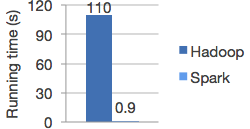
\includegraphics[width=\linewidth]{spark_time.png}
\end{columns}

\vfill
\begin{itemize}
\item I primarily used Hadoop in industry, but I've working more with Spark recently.
\item In addition to the speedup, Spark has many minor conveniences. It's made for data analysts!
\item Spark also generalizes to streams of composed functional primitives, not just map and reduce.
\end{itemize}
\end{frame}

\begin{frame}[fragile]{Functional primitives}

A functional programming style is preferred by data analysts using R (inherited from Scheme) and Spark (inherited from Scala).

\begin{columns}
\column{0.6\linewidth}
\begin{lstlisting}[language=c,frame=single]
for (i = 0;  i < nEvents;  i++) {
    event = events(i);
    if (condition(event))
        continue;
    add_to_output(calculation(event));
}
\end{lstlisting}
\column{0.42\linewidth}
\begin{lstlisting}[language=python,frame=single]

output =
  events.filter(condition)
        .map(calculation)


\end{lstlisting}
\end{columns}

\begin{itemize}
\item The ``map'' call says less than ``for''--- it doesn't specify an order in which events must be processed.
\item Underlying system can distribute and collect however it likes.
\item Also doesn't involve the user in indexing over subsets of data, which can be error-prone.
\end{itemize}
\end{frame}

\begin{frame}{``Monad'' operations:}

Transforming one data table (ntuple) into another.

\vfill
\renewcommand{\arraystretch}{1.5}
\begin{tabular}{p{0.12\linewidth} >{\centering}p{0.08\linewidth} >{\centering}p{0.17\linewidth} >{\centering}p{0.08\linewidth} p{0.4\linewidth}}
& input & function & output & operation \\\hline
\textcolor{darkblue}{map} & table of $A$ & $f: A \to B$ & table of $B$ & apply $f$ to each row $A$, get a table of the same number of rows $B$ \\
& \multicolumn{4}{l}{\scriptsize \color{darkgrey} a.k.a. ``lapply'' (R), ``SELECT'' (SQL), list comprehension (Python)} \\
\textcolor{darkblue}{filter} & table of $A$ & $f: A \to \mbox{boolean}$ & table of $A$ & get a shorter table with the same type of rows \\
& \multicolumn{4}{l}{\scriptsize \color{darkgrey} a.k.a. single brackets (R), ``WHERE'' (SQL), list comprehension (Python)} \\
\textcolor{darkblue}{flatMap} & table of $A$ & $f: A \to \mbox{table of } B$ & table of $B$ & compose \textcolor{darkblue}{map} and \textcolor{darkblue}{flatten}, get a table of any length \\
& \multicolumn{4}{l}{\scriptsize \color{darkgrey} a.k.a. ``map'' (Hadoop), ``EXPLODE'' (SQL), $>>=$ (Haskell)} \\
\end{tabular}
\end{frame}

\begin{frame}{``Monoid'' operations:}

Summarizing an ntuple with a counter or a histogram.

\vfill
\renewcommand{\arraystretch}{1.5}
\begin{tabular}{p{0.12\linewidth} >{\centering}p{0.2\linewidth} >{\centering}p{0.23\linewidth} >{\centering}p{0.08\linewidth} >{\raggedright\arraybackslash}p{0.25\linewidth}}
& input & function(s) & output & operation \\\hline
\textcolor{darkblue}{reduce} & table of $A$ & $f: (A, A) \to A$ & single $A$ & apply $f$ to the running sum and one more element \\
\textcolor{darkblue}{aggregate} & table of $A$, initial value $B$ (``zero'') & $f: (A, B) \to B$ $f: (B, B) \to B$ (increment and combine) & single value $B$ & accumulate a counter with a different data type from the input \\
\textcolor{darkblue}{aggregate by key} & table of $\langle K,A \rangle$, initial value $B$ & $f: (A, B) \to B$ $f: (B, B) \to B$ & pairs $\langle K,B \rangle$ & aggregate independently for each key \\
& \multicolumn{4}{l}{\scriptsize \color{darkgrey} a.k.a. ``reduce'' (Hadoop), ``GROUP BY'' (SQL)} \\
\end{tabular}
\end{frame}

\begin{frame}{Associativity is key}

``Monad'' and ``monoid'' refer to mathematical properties of the operator, the most important being associativity, which allows the inputs to be dispatched arbitrarily.

\begin{center}
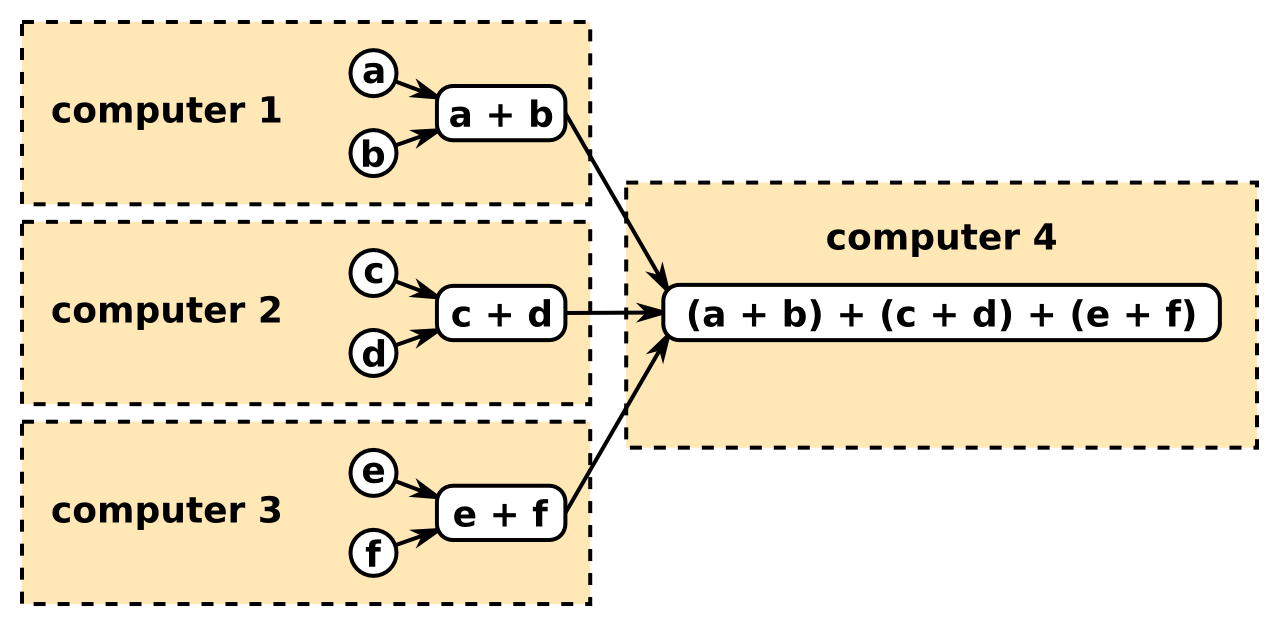
\includegraphics[width=0.7\linewidth]{monoids.png}
\end{center}

Commutativity is nice, too, because then the system doesn't have to worry about the order in which they're combined.
\end{frame}

\begin{frame}[fragile]{Histograms in a functional context}

A histogram is a counter, which obeys monoid rules because
\begin{itemize}
\item it has an identity element (empty histogram),
\item it has an associative binary operation (histogram addition).
\end{itemize}

\vfill
It fits very naturally into Spark's \textcolor{darkblue}{aggregateByKey} functional:

\begin{lstlisting}[language=scala]
val parallel_histogram_result =
    dataset.aggregate(new TH1F(100, 0.0, 50.0))(   // booking
        {(hist, datum) => hist.Fill(datum)},       // filling
        {(hist1, hist2) => hist1.Add(hist2)})      // combining
\end{lstlisting}

\vfill
\begin{uncoverenv}<2->
However, this becomes cumbersome for a large number of histograms: we'd have to maintain the list of histograms as inputs and outputs of three different functions.

\vfill
Ideally, we'd want a ``collection of histograms'' (also a monoid) to pass to \textcolor{darkblue}{aggregateByKey} for Spark to update all at once.
\end{uncoverenv}
\end{frame}

\begin{frame}{Histograms in a functional context}

So we make {\tt Pack\_O\_Histograms}, a mapping from string names to histograms, with methods to iterate over its contents, applying {\tt Fill} and {\tt Add} to each.

\vfill
However, {\tt Pack\_O\_Histograms} is a bit like a meta-histogram, where the string names are the bins of the meta-histogram.

\vfill
What if a particularly complex analysis wanted packs of {\tt Pack\_O\_Histograms}?
\end{frame}

\begin{frame}{Histograms in a functional context}

Consider instead breaking histograms down into its fundamental primitives:
\begin{itemize}
\item {\tt Counter} just counts.
\item {\tt MeanRms} accumulates a mean and RMS.
\item {\tt Binned(f, Counter)} is a standard 1-d histogram with a fill rule $f$. (Declare how it gets filled at booking-time.)
\item {\tt Binned(f, MeanRms)} is a ``profile plot.''
\item {\tt Binned(f, Binned(g, Counter))} is a standard 2-d histogram with a fill rule $f$ for x and $g$ for y.
\item {\tt Mapping(Binned(f, Counter))} is a pack of histograms.
\item {\tt Conditions([a, b, c], Binned(f, Counter))} is a suite of histograms filled under conditions $a$, $b$, and $c$.
\item and any other algebraic combination\ldots
\end{itemize}
\end{frame}

\begin{frame}{Histograms of histograms are already a common tool}

But currently, the aggregation is performed using imperative analysis scripts with containers designed around their graphical representations.

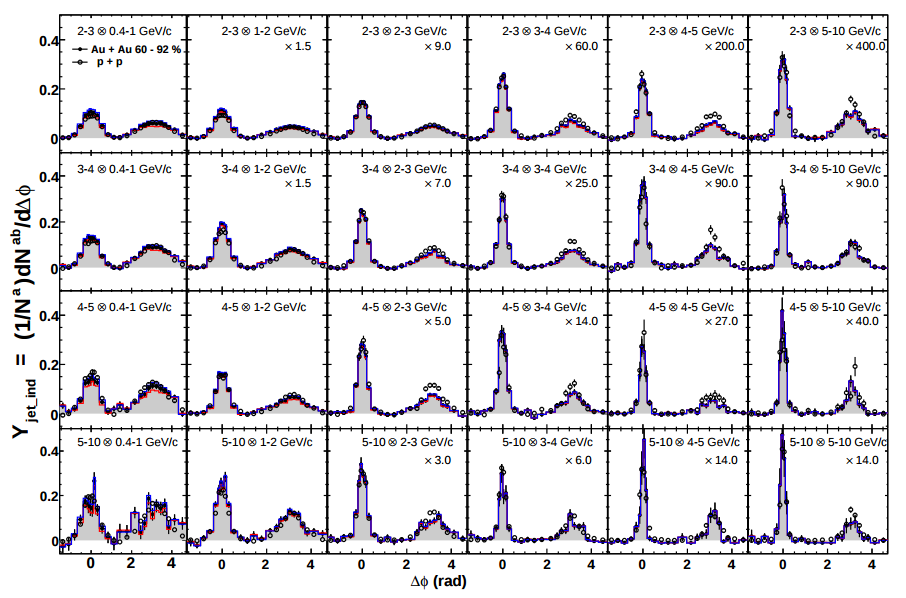
\includegraphics[width=\linewidth]{histograms_of_histograms.png}
\end{frame}

\begin{frame}{Conclusions}

Hopefully, this talk got you thinking about how {\it your} problems could be solved with Big Data tools:
\begin{itemize}
\item Code maintenance by a large community of software engineers.
\item Data transposition (the ``reduce'' step in map-reduce).
\item Resilient stream processing, which I didn't talk about.
\item Data-handling abstractions such as those used in R and Spark.
\end{itemize}

\vfill
If so, please tell me your ideas! Maybe we can build something together.
\end{frame}

\end{document}
